\chapter[Player/Stage/Gazebo ]{Player/Stage/Gazebo \label{chap:gazebo}}
\chaptermark{Player/Stage/Gazebo}
	Symulator \mbox{\texttt{Player/Stage/Gazebo}} został już opisany w pracy inżynierskiej \cite{inzynierka} jednak z uwagi na jego ważną rolę i zmiany jakie zdecydowano się wprowadzić w symulowanym
	środowkisku podczas rozwijania aplikiacji zdecydowano się na krótkie przypomnienie koncepcji projektu.

	\section{Koncepcja}
	Początki oprogramowania nazwanego \textit{Project Player} (oznaczającego zestaw trzech aplikacji: \textit{Player}, \textit{Stage} oraz \textit{Gazebo}) 
	sięgają 1998 roku, kiedy to
 	na Uniwersytecie Południowej Kaliforni w Los Angeles rozpoczęto prace nad stworzeniem oprogramowania pozwalającego 
 	na sterowanie grupą robotów mobilnych \textit{Pioneer~2} firmy ActivMedia, będących na wyposażeniu tamtejszego laboratorium robotyki. 
	Twórcami projektu byli Brian Gerkey i Richard Vaughan, później dołaczyli do nich Kasper St{\o}y oraz Andrew Howard.
	Do tego czasu w skład stworzonego oprogramowania wchodziły: \textit{Golem} (pozwalający na sterowanie
	robotem \textit{Pioneer}) oraz \textit{Arena} (symulator). W toku prac narodziła się idea opracowania uniwersalnego zestawu aplikacji, umożliwiającego kontrolę nad robotami niezależnie od zastosowanych rozwiązań sprzętowych, 
	dobrze współpracującego z symulatorem oraz dostępnego za darmo (zgodnie z GNU GPL). 
	Tak powstały aplikacje \textit{Player} oraz \textit{Stage}. \textit{Player} miał za zadanie dostarczać narzędzi do sterowania podzespołami robota, 
	a \textit{Stage} stanowił prosty dwuwymiarowy symulator. Oprogramowanie to znalazło szeroko stosowane 
	zarówno w uczelnianych laboratoriach, jak i wśród indywidualnych użytkowników. W 2002 roku rozpoczęto prace
	nad nowym symulatorem \textit{Gazebo}, który miał służyć do modelowania zachowań robotów w trójwymiarowym świecie 
	z uwzględnieniem rzeczywistych oddziaływań fizycznych między obiektami. Całość projektu jest w dalszym ciągu intensywnie rozwijana przez
	deweloperów oraz aktywną społeczność użytkowników. Oprogramowanie działa na systemach Linux, Solaris, *BSD oraz Mac OSX. 
	Szczegółowe informacje, dokumentacja oraz kody źródłowe każdej z aplikacji dostępne są pod adresem \url{http://playerstage.sourceforge.net/}.
	W trakcie prac nad opisywaną aplikacją wydana została stabilna wersja symulatora i zmieniona strona internetowa projektu, obecnie jest on dostępny pod \url{http://gazebosim.org/}.
	
	\section{Architektura symulatora}
	\begin{figure}[!b]
	\centering
	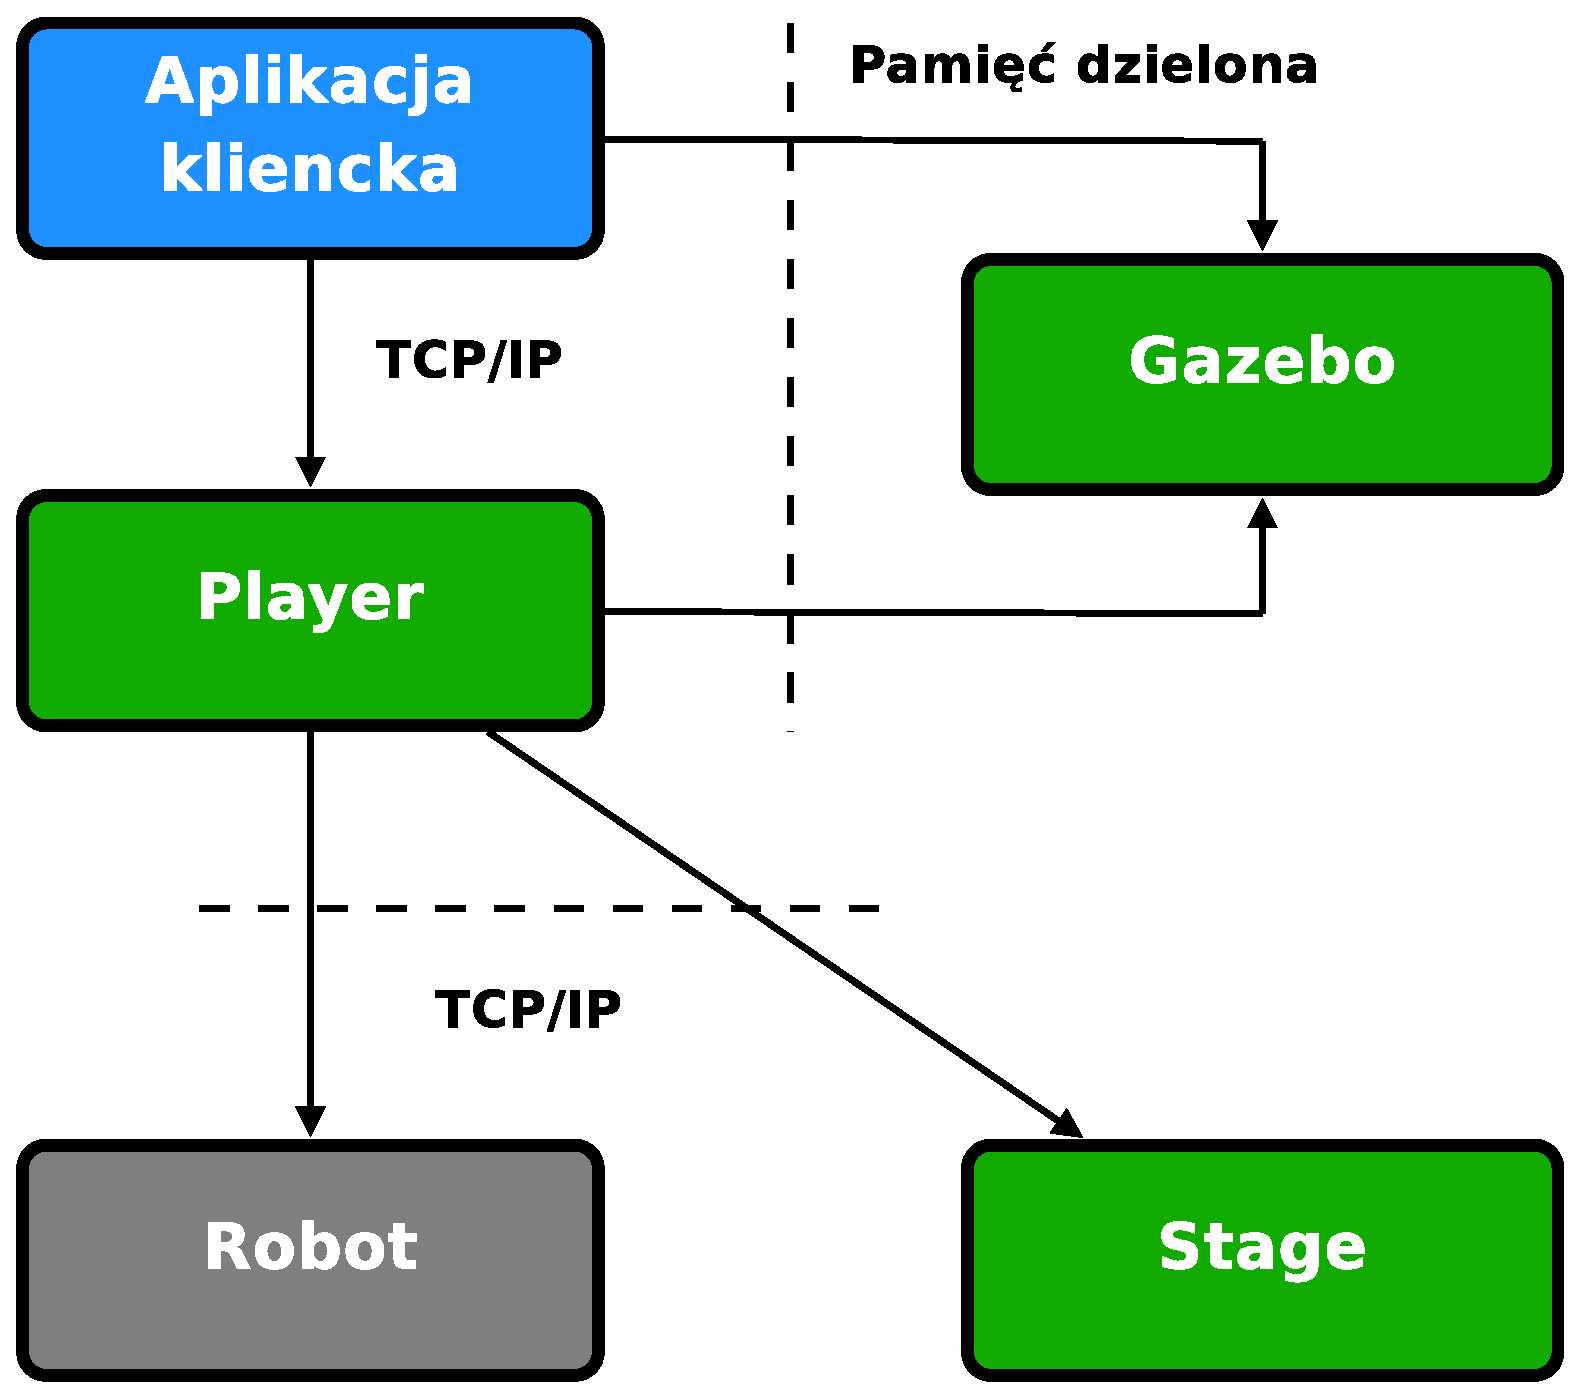
\includegraphics[scale=0.3]{./gazebo/architektura}
	\caption{Schemat komunikacji w środowisku \textit{Player/Stage/Gazebo} \label{fig:arch}}
	\end{figure}
	
	Schemat zależności pomiędzy komponentami \textit{Player/Stage/Gazebo} został przedstawiony na 
	rysunku~\ref{fig:arch}.
	Dobrze obrazuje on rolę programu \textit{Player}, pełniącego funkcję pośrednika pomiędzy aplikacją klienta 
	(odpowiadającą za algorytm sterowania robotem) a rzeczywistym robotem lub symulatorami modelującymi jego zachowanie (\textit{Stage} oraz \textit{Gazebo}). Do komunikacji 
	pomiędzy komponentami wykorzystywany jest protokół TCP/IP. Aplikacja kliencka łączy się z ``serwerem'', którego
	rolę pełni \textit{Player}. Z punktu widzenia klienta nie ma znaczenia, czy interfejsy dostarczane przez \textit{Playera} sterują robotem rzeczywistym,
	czy tylko jego wirtualnym odpowiednikiem (modelem) w jednym z symulatorów. Ponadto, przeniesienie kontroli
	pomiędzy symulowanym a rzeczywistym robotem wymaga tylko nieznacznych modyfikacji kodu.

	Istnieje jeszcze druga opcja -- do każdego z symulatorów (\textit{Stage} lub \textit{Gazebo}) można odwoływać się bezpośrednio w przypadku,
	gdy korzystanie z \textit{Playera} nie jest uzasadnione, lub gdy chce się dokonać pewnych modyfikacji w sposobie
	działania symulatora. Do tego celu zostały stworzone biblioteki (\textit{libstage} oraz \textit{libgazebo}), 
	które dostarczają funkcji służących do komunikacji między aplikacją kliencką, a symulatorami.
	\begin{figure}[h]
	\centering
	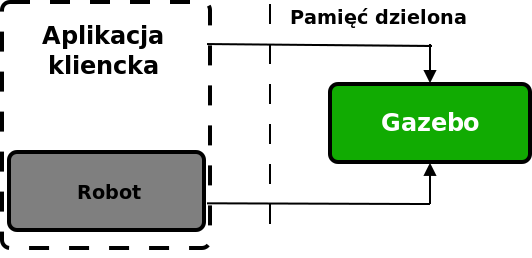
\includegraphics[scale=0.3]{./gazebo/wybrana_architektura}
	\caption{Zrealizowany schemat komunikacji w środowisku \textit{Player/Stage/Gazebo} \label{fig:wybrana_arch}}
	\end{figure}
	Podsumowując, struktura pakietu oprogramowania \mbox{\textit{Player/Stage/Gazebo}} umożliwia tworzenie aplikacji sterujących robotami w sposób, który zapewnia przenośność stworzonych programów i ich działanie zarówno na symulatorach robotów, jaki i na rzeczywistych obiektach.
	
 	\subsection{Gazebo}
 	
 	Program \textit{Gazebo}, podobnie jak \textit{Stage}, umożliwia symulację grup robotów mobilnych. Różnica polega na tym, że symulowane
 	środowisko jest trójwymiarowe, uwzględnia dynamikę, cechy fizyczne oraz oddziaływania między modelami. Wiąże się
 	to oczywiście ze wzrostem potrzebnej mocy obliczeniowej, dlatego też symulowane grupy robotów nie
 	mogą być tak liczne, jak w przypadku \textit{Stage}.
 	 	
 	\textit{Gazebo} zostało oparte na nastepujących komponentach:
 	\begin{itemize}
 	 \item ODE\footnote{Open Dynamics Engine, \url{http://www.ode.org}}, bibliotece  odpowiadającej za symulację
 	 	cech fizycznych brył oraz detekcję kolizji,
 	 \item OGRE\footnote{Object-Oriented Graphics Rendering Engine, \url{http://www.ogre3d.org/}}, 
		silniku graficznym umożliwiającym tworzenie wspomaganej sprzętowo grafiki 3D,
 	 \item FLTK\footnote{Fast Light Toolkit, \url{http://www.fltk.org/}}, bibliotece dostarczającej 
		przenośny interfejs użytkownika dla Gazebo,
	 \item libXML2\footnote{ \url{http://xmlsoft.org/}}, parserze XML (stworzonym oryginalnie dla środowiska graficznego GNOME), umożliwiającym Gazebo proste wczytywanie plików konfiguracyjnych.
 	\end{itemize}

	\textit{Gazebo} pozwala na symulację standardowych sensorów (m.in. czujniki odległości, kamery, GPS). Dostarcza gotowe modele 
	popularnych robotów (jak np. \textit{Pioneer2DX}, \textit{Pioneer 2AT} oraz \textit{SegwayRMP}). Pozwala ponadto na tworzenie własnych modeli
	i definiowanie ich własności fizycznych (takich jak np. masa, współczynnik tarcia, sztywność), co zapewnia odpowiedni realizm
	symulacji i pozwala na interakcję z innymi obiektami (podnoszenie, przesuwanie brył itp.). Co więcej, dla każdego z modeli
	dostępne są kontrolery pozwalające na ich sterowanie, ale nic nie stoi na przeszkodzie, żeby zdefiniować własne według potrzeb i dodać je do \textit{Gazebo}. 
	\begin{figure}[!t]
	\centering
	\label{fig:gazebo}
	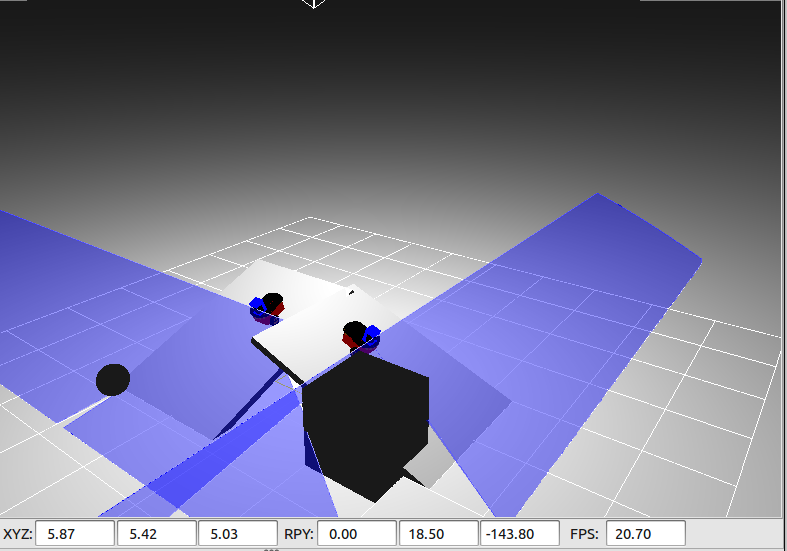
\includegraphics[scale=0.42]{./gazebo/gazebo_screen}
	\caption{\textit{Gazebo} -- okno główne (wersja 0.10)}
	\end{figure}

	\section{Modelowanie obiektów w Gazebo}
	Filozofia modelowania w \textit{Gazebo} opiera się na tworzeniu opisu świata (o parametrach określonych 
	w pliku \textit{.world} za pomocą języka XML), w którym umieszczone zostają symulowane obiekty. Plik zawiera informacje o dodanych do świata modelach, ale także parametry określające przebieg symulacji, takie 
	jak krok pracy symulatora czy sposób detekcji kolizji. 
	\subsection{Zasady modelowania w Gazebo 0.10}
	Opis modelowanego świata powinien zawierać się w pliku głównym z rozszerzeniem \textit{.world}.
	W pliku muszą być zapisane informacje związane z konfiguracją interfejsu użytkownika, sposobem renderowania sceny oraz fizyką symulacji.
	Elementy przykładowego pliku \textit{.world} zostały zaprezentowane na listingach poniżej.
	%\small
	%\lstset{language=XML,  basicstyle=\ttfamily\footnotesize,
	\lstset{language=XML,  basicstyle=\ttfamily\scriptsize, 
	commentstyle={}, xleftmargin=20pt, numbers=left, numberstyle=\footnotesize,
	caption={},
	backgroundcolor=\color{light-gray},
	frame=single,
	breaklines=true}
	\begin{lstlisting}[name=gazebo_simple_world]
	<?xml version="1.0"?>
	<gazebo:world>
	\end{lstlisting}
	Bardzo istotnym elementem jest konfiguracja fizyki (ODE), interfejs umożliwia konfigurację globalnych parametrów takich jak:
	\begin{lstlisting}[name=gazebo_simple_world]
	<physics:ode>
		<stepTime>0.001</stepTime>
		<gravity>0 0 -9.8</gravity>		
		<erp>0.8</erp>
		<cfm>0.05</cfm>
		<stepType>quick</stepType>
		<stepIters>25</stepIters>
		<stepW>1.4</stepW>
		<contactSurfaceLayer>0.007</contactSurfaceLayer>
		<contactMaxCorrectingVel>100</contactMaxCorrectingVel>
	 </physics:ode>
	\end{lstlisting}
	\lstset{language=XML,  basicstyle=\ttfamily\footnotesize, 
	commentstyle={}, xleftmargin=20pt, numbers=left, numberstyle=\footnotesize,
	caption={},
	backgroundcolor=\color{light-gray},
	frame=single,
	breaklines=true}
	Znaczenie poszczególnych parametrów jest następujące:
	\begin {enumerate}
	 \item \texttt{stepTime} jest wyrażony w sekundach i określa czas pomiędzy kolejnymi aktualizacjami silnika \texttt{ODE},
	 \item \texttt{gravity} jest wektorem określającym siłę grawitacji,
	 \item \texttt{erp} rozwija się na \textit{error reduction parameter}, przyjmuje on wartości z przedziału od $0$ do $1$ i jest odpowiedzialny za redukcję błędów w połączeniach pomiędzy bryłami
	  (problematyka zostanie szerzej poruszona na stronie \pageref{fig:joints}); \texttt{erp} ustawione na $0$ powoduje, że żadna dodatkowa siła nie jest przykładana do danej bryły, natomiast wartość $1$
	 powoduje, że wszytskie błędy połączeń zostaną naprawione w kolejnym kroku symulatora,
	 \item \texttt{cfm} jest skrótem od \textit{constraint force mixing} i odpowiada za sztywność ograniczeń występujacych w kolizjach między bryłami, gdy wartość jest równa $0$ ograniczenie wynikające z fizyki
nie może zostać złamane, ustawienie parametru na wartość dodatnią powoduje, że ograniczenie staje się ``miękkie'', sprężyste,
	  
	 \item \texttt{stepType} odpowiada za rodzaj używanej funkcji z \texttt{ODE} do detekcji kolizji, użytkownik może dokonać wybrou jednej z dwóch wartości:
	      \begin{itemize}
	       \item \textit{world}, używana jest wtedy funkcja \texttt{dWorldStep}, operująca na macierzy zawierającej wszystkie ograniczenia, złożoność obliczeniowa tej metody wynosi $m^3$, natomiast pamięciowa
jest rzędu $m^2$, gdzie $m$ określa ilość wierszy (ograniczeń) analizowanej macierzy,
	       \item \textit{quick}, do detekcji kolizji stosowana jest metoda iteracyjna, w literaturze nazywana \texttt{SOR - Successive over-relaxation} należąca do rodziny metod Gaussa–Seidela, jej złożoność obliczeniowa jest rzędu $m*N$,
		a pamięciowa $m$, gdzie $m$ ma znaczenie jak wyżej,
		natomiast $N$ jest liczbą iteracji; dla dużych systemów metoda jest dużo bardziej wydajna jednak mniej dokładna, mogą także występować problemy z jej stabilnością; najprostszą metodą na poprawę stabilności
		jest zwiększanie \texttt{cfm}, 
	      \end{itemize}
	 \item \texttt{stepIters} - ilość iteracji, gdy do detekcji kolizji wybrano metodę \textit{quick},
	 \item \texttt{stepW} określa czas relaksacji metody Gaussa–Seidela, 
	 \item \texttt{contactSurfaceLayer} określa głębokość na jaką może wnikać bryła w podłoże, ustawienie parametru na małą wartość dodatnią zapobiega jitterowi w momencie, gdy ograniczenia są nieustannie tworzone
	  i zrywane (na przykład podczas ruchu koła po podłożu),
	 \item \texttt{contactMaxCorrectingVel} jest maksymalną korektą prędkości jaka może wynikać z utworzonych tymczasowo kontaktów; domyślnie parametr przyjmuje nieskończoną wartość.
	  \todo{przetlumaczyc na polski}Reducing this value can help prevent "popping" of deeply embedded objects. 
	\end {enumerate}
	Warto wspomnieć, że niektóre parametry można zmieniać dla poszczególnych modeli lub połączeń \textit{joints}.\newline
	Ustawienia interfejsu: typ (dostępne tylko \textit{fltk}), rozmiaru okna i jego pozycja początkowej:
\begin{lstlisting} [name=gazebo_simple_world]
    <rendering:gui>
        <type>fltk</type>
        <size>640 480</size>
        <pos>0 0</pos>
    </rendering:gui>
\end{lstlisting}
	Określenie parametrów renderowanej sceny: techniki cieniowania, tekstury pokrywającej niebo (dostępne inne opcje, jak np. rodzaje oświetlenia, dodawanie mgły itp.):
\begin{lstlisting} [name=gazebo_simple_world]
    <rendering:ogre>
        <shadowTechnique>stencilAdditive</shadowTechnique>
        <sky>
              <material>Gazebo/CloudySky</material>
        </sky>
    </rendering:ogre>
</gazebo:world>
\end{lstlisting}

	Do tak stworzonego pliku z opisem świata należy następnie dodać modele.  Dodany obiekt musi zawierać co najmniej jeden element \textit{body}, który jest złożony z elementów \textit{geoms}. Sekcja opisująca przykładowy model piłki mogłaby wyglądać następująco:
	\begin{figure}[H]
	\centering
	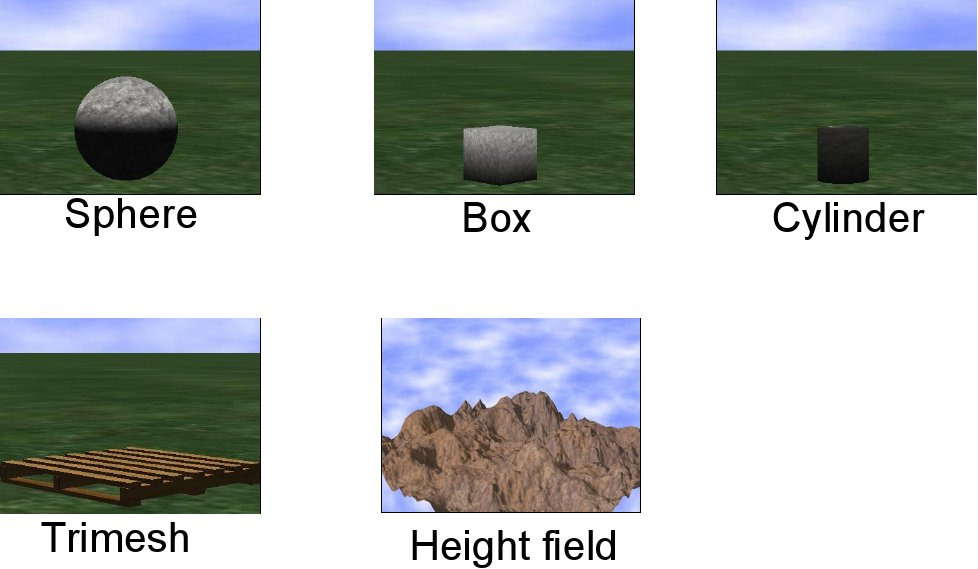
\includegraphics[scale=0.35]{./gazebo/geoms}
	\caption[Dostępne typy \textit{geoms}]
		{\label{fig:geoms}Dostępne typy \textit{geoms} -- Gazebo 0.10 (źródło:~\cite{gazebo_experts})}
	\end{figure}
	
	\lstset{language=XML,  basicstyle=\ttfamily\footnotesize, 
	commentstyle={}, xleftmargin=20pt, numbers=left, numberstyle=\footnotesize,
	caption={},
	backgroundcolor=\color{light-gray},
	frame=single,
	breaklines=true}
\begin{lstlisting}[name=gazebo_przyklad_pilka]
<model:physical name="ball">
    <static>false</static>
\end{lstlisting}
Na wstępie deklarowany jest model, którego parametr \textit{static} ustawiono na \textit{false}, co oznacza, że będzie on brał udział
w symulacji fizycznej i może oddziaływać z innymi obiektami. Następnie należy zadeklarować ``ciało'' tworzonego obiektu:
\begin{lstlisting}[name=gazebo_przyklad_pilka]
    <body:sphere name = "ball_body">	
\end{lstlisting}
Wewnątrz \textit{body}, które jest odpowiedzialne za dynamikę obiektu, należy umieścić elementy opisujące kształt obiektu (pozwalające tym samym na detekcję kolizji) -- w tym przypadku zdefiniowano kulę o wymiarach i masie odpowiadającej piłce do golfa:
\begin{lstlisting}[name=gazebo_przyklad_pilka]
	<geom:sphere name = "ball_geom">
		<xyz>0 0 0.01</xyz>
		<rpy>0 0 0 </rpy>
		<size>0.02</size>
		<mass>0.045</mass>
\end{lstlisting}
Sekcja \textit{visual} bloku \textit{geom} pozwala na przypisanie obiektowi wyglądu -- może to być figura o dowolnym kształcie (stworzona np. w programie do grafiki 3D) i wybranej przez projektanta teksturze lub kolorze:
\begin{lstlisting}[name=gazebo_przyklad_pilka]
		<visual>	
			<scale>0.02 0.02 0.02</scale>
			<size>0.02</size>
			<mesh>unit_sphere</mesh>
			<material>Gazebo/Orange</material>
		</visual>
	</geom:sphere>				
    </body:sphere>
</model:physical>
\end{lstlisting}	


	
	\subsubsection{Połączenia pomiędzy bryłami }
	Tworząc modele, można korzystać z trzech podstawowych brył (kula, walec, prostopadłościan), a także z siatek \textit{trimesh} oraz elementów \textit{height field} (stworzonych do generowana terenu -- por. rys. \ref{fig:geoms})).
	Żeby zamodelować robota, należy jeszcze stworzone bryły odpowiednio ze sobą powiązać. Do tego służą elementy typu \textit{joint}, którymi można łączyć komponenty \textit{body} (modelujące np. koła i podwozie robota).
	Stopnie swobody połączenia zależą od wybranego typu wiązania \textit{joint} (dostępne typy przedstawiono na rys. \ref{fig:joints}). Obiekty połączone wiązaniem tworzą parę kinematyczną.
	\textit{Gazebo} umożliwia nadawanie tak połączonym bryłom prędkości obrotowych względem siebie, co pozwala na modelowanie ruchomych elementów robotów.
	\begin{figure}[H]
	\centering
	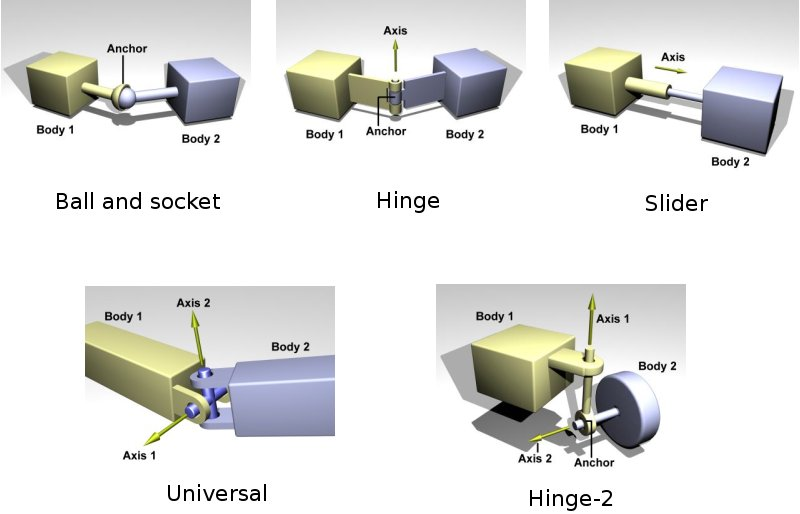
\includegraphics[scale=0.43]{./gazebo/joints}
	\caption{Typy połączeń \textit{joints} (Źródło: dokumentacja ODE) \label{fig:joints}}
	\end{figure}
	Jak wspomniano wcześniej, w czasie realizowanej symulacji połączenia pomiędzy bryłami moga ulec wypaczeniu, na skutek sił działających na model. Może to być tarcie,
	siła powodująca obrót bryły czy siły działające na model podczas kolizji. Sytacje taką przedstawiono na rysunku \ref{fig:bad_joint}.
	\begin{figure}[H]
	\centering
	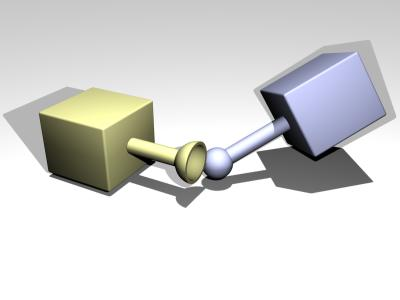
\includegraphics[scale=0.43]{./gazebo/bad_joint}
	\caption{Zepsute połączenie (\textit{joints}) (Źródło: dokumentacja ODE) \label{fig:bad_joint}}
	\end{figure}
	Błędy tego typu można redukować za pomocą parametru \texttt{erp} ustawianego globalnie lub dla każdego z połączeń indywidualnie.
	\subsubsection{Sterowniki modeli }
	Sterowanie zaprojektowanym modelem jest możliwe po uprzednim wyposażeniu go w sterownik (\textit{controller}). Sterowniki implentowane są przez użytkownika w $C++$ jako klasa dziedzicząca
	po zdefiniowanym w \textit{libgazebo} interfejsie. Klasa odpowiada za przetwarzanie danych z sensorów robota oraz pozwala
	na zadawanie prędkości bryłom połączonym wiązaniami. Komunikuje się on z programem sterującym za pośrednictwem interfejsów (bezpośrednio korzystając z \textit{libgazebo} lub poprzez \textit{Playera}).
	\textit{Gazebo} oczywiście dostarcza gotowe sterowniki, pozwalające na kontrolowanie np. robota z napędem różnicowym, w wersji $0.10$ dodano także przykładowy model robota holonomicznego zawarty
	w pliku \textit{wizbot.world}. Aby z nich skorzystać, wystarczy przypisać wybrany sterownik do modelu robota, określić, które ze złączeń odpowiadają jego kołom i podać nazwę instancji interfejsu,
	za pomocą którego odbywać ma się komunikacja pomiędzy klientem a sterownikiem. W przypadku sterowania przemieszczeniem będzie to interfejs \textit{position}, za pomocą którego możemy zadawać prędkości bryłom,
	ale \textit{Gazebo} posiada też zaimplementowane interfejsy do sterowania innymi elementami np. do komunikacji z laserowymi czujnikami odległości, kamerą bądź chwytakiem manipulatora. 
	\lstset{language=XML,  basicstyle=\ttfamily\footnotesize, 
	commentstyle={}, xleftmargin=20pt, numbers=left, numberstyle=\footnotesize,
	caption={Przykład przypisanie sterownika do modelu},
	backgroundcolor=\color{light-gray},
	frame=single,
	breaklines=true}
	\begin{lstlisting}
<model:physical name="pioneer_model">
    <controller:pioneer2dx_position2d name="controller">
        <leftJoint>left_hinge_joint</leftJoint>
        <rightJoint>right_hinge_joint</rightJoint>
        <interface:position name="position_iface"/>
    </controller>
</model:physical>
	\end{lstlisting}	

	
	\subsection{Realizacja środowiska Ligi RoboCup \label{subsect:realizacjaROBOCUP} }
	
	W celu realizacji niniejszej pracy stworzono dla symulatora \textit{Gazebo} modele odpowiadające robotom biorącym udział w \emph{Small-size League}. 
	Boisko zostało stworzone z wykorzystaniem rzeczywistych wymiarów($5.4[m] x 7.4[m]$). 
	Zgodnie z regułami Ligi z 2007 roku\protect\footnote{\url{http://small-size.informatik.uni-bremen.de/rules/f180rules2007.html}} utworzono również linie boiska, 
	pozostawiając wystarczającą dla robota przestrzeń przy bandach tak, żeby było możliwe np. wykonywanie zagrań z autu. 
	Model piłki odpowiada piłce do golfa, której używa się w oficjalnych rozgrywkach.
	
	\begin{figure}[!b]
	\centering
	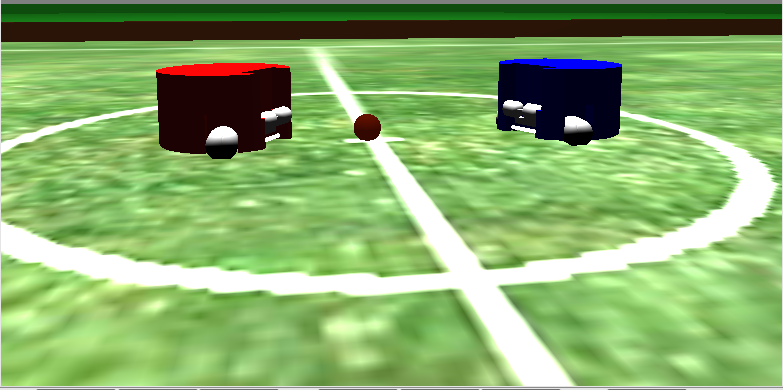
\includegraphics[scale=0.4]{./gazebo/roboty}
	\caption{Opracowane modele robotów (oparte na konstrukcji HMT)}
	\end{figure}

	Wykonane modele robotów wzorowano na konstrukcji rzeczywistych robotów wykorzystywanych w \emph{Small-size League}.
	Główna częścią robota jest walec o promieniu $6[cm]$ i wysokości $4[cm]$, umieszczony na trzech kołach rozmieszczonych symetrycznie na podstawie walca.
	Robot został dodatkowo wyposażony w \textit{dribbler}\protect\footnote{urządzenie opisano w par.~\ref{sec:budowa_robota}} pomagający utrzymać kontrolę nad piłką.
	Mimo że \textit{Gazebo} udostepnia sterownik dla napędu holonomicznego, sterowanie robotem wymagało napisania nowego kontrolera, ponieważ nie uwzględniał on obsługi
	\textit{dribblera}. Kod źródłowy sterownika został zamieszczony na płycie CD razem z kodem źródłowym wykorzystywanej wersji symulatora.	
	\begin{figure}[H]
	\centering
	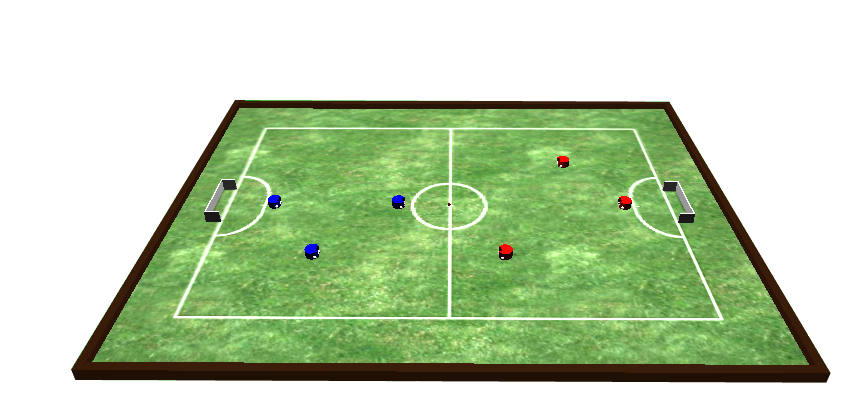
\includegraphics[scale=0.4]{./gazebo/boisko.png}
	\caption{Model boiska}
	\end{figure}

	W trakcie prac nad modelowaniem Ligi wprowadzono kilka poprawek w symulatorze. Aby zamodelować w pełni koło szwedzkie należało dodać możliwośc określenia
	w jakim kierunku dla danej bryły występuje tarcie. W tym celu w skecji opisującej bryłę dodano nowy parametr:
	\lstset{language=XML,  basicstyle=\ttfamily\footnotesize, 
	commentstyle={}, xleftmargin=20pt, numbers=left, numberstyle=\footnotesize,
	caption={Parametr określający kierunek siły tarcia},
	backgroundcolor=\color{light-gray},
	frame=single,
	breaklines=true}
	\begin{lstlisting}	
	<fDir1>1 0 0</fDir1>
	\end{lstlisting}
	Powyższa wartość oznacza, że tarcie występuje jedynie w kierunku osi $OX$ danej bryły.
	\todo{opisac jak zaimplentowano w ode brak tarcia}